\chapter{TestBeam setup}

%%% motivate testbeam
A typical way to test sensors for High-Energy Physics applications is to put the Devices Under Test (DUTs) through a focused flux of high energy particles and then to read out and analyze the response, a.k.a. test beam.

The HGTD collaboration has conducted many test beam campaigns, mainly at CERN and at DESY (Deutsches Elektronen-Synchrotron). The focus of this analysis is the test beam campaign of May 2023, performed at CERN using a beam of \qty{120}{\giga\electronvolt} pions, provided by SPS.
The experimental setup of this campaign included: 
\begin{itemize}
    \item Trigger Logic Unit (TLU), it provided an event trigger, from the signal of a scintillator. %% describe trigger??
    \item FE-i4, it selected a Region Of Interest (ROI), a HitOR for the trigger, to avoid noisy pixels.
    \item 6 MIMOSA planes, they measured the position of the particles in the beam, enabling track reconstruction.
    \item Microchannel Plate detector (MCP), it was used as reference for the time resolution.
    \item Cooling box containing the various DUTs, mantained at \qty{-30}{\degreeCelsius}.
    \item 2 oscilloscopes acquired the data from the MCP (Channel 1) and the DUTs (Channels 2,3 and 4).
\end{itemize}

%%% maybe this should just be later
The main quantities of interest were: time resolution, the collected charge and the hit efficiency.

In this setting different variations of LGADs were tested: with different manufacturers, different radiation doses and different designs.
%%% what are the main things tested for: time resolution, charge, efficiency, impact of radiation.

\begin{figure}[!ht]
    \centering
    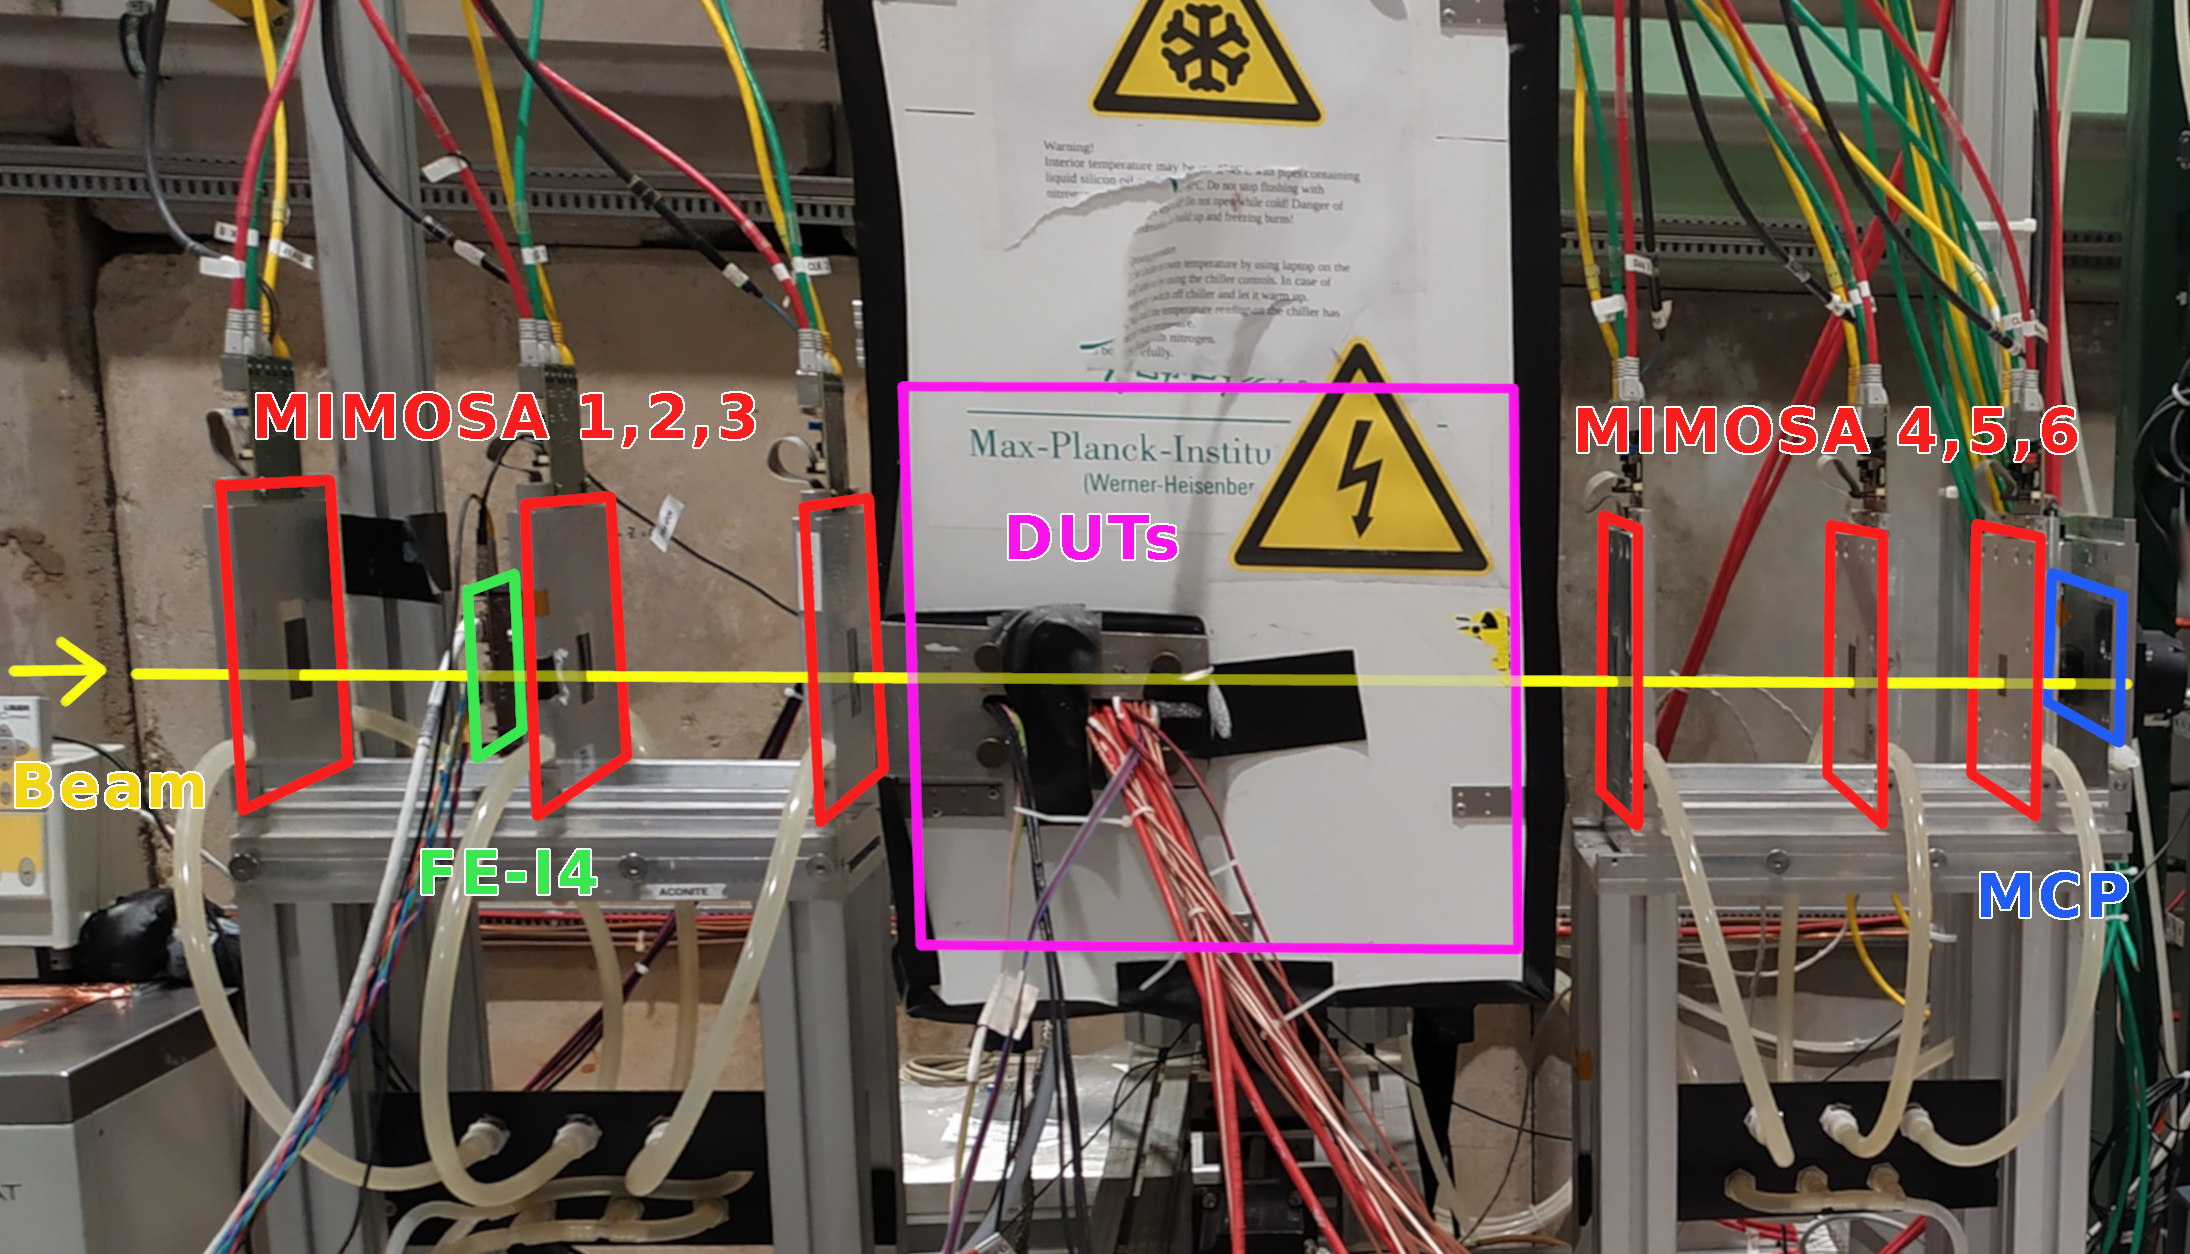
\includegraphics[width=.95\linewidth]{Images/TestBeam_setup/TestBeam_setup_redrawn.png}
    \captionsetup{width=.8\linewidth}
    \caption{The components of the TestBeam setup: six MIMOSA planes, the FE-I4, the MCP and the cooling box containing the DUTs}
    \label{fig:testbeam_setup}
\end{figure}

% description of components:
% • Trigger logic unit for particle passing
% • FEi4 to select a region of interest
% • Mimosa planes for tracking (X and Y position data)
% • MCP for time reference 
% • Cooling box containint the DUTs, (can be tilted with respect to the beam direction)
% • 120 GeV beam of pion
\section{TLU and FEi4}

more description of FE-i4.
Region of interest, show plots
problems with that \marginpar{\flushleft maybe should be in the appendix}

The Trigger Logic Unit received the signal from a scintillator and the HitOR\footnote{A binary signal generated when \textbf{at least one pixel} registers a hit} from the FE-i4 and provided a trigger for the data acquisition.

\section{MIMOSA planes}

A total of 6 planes 
576 rows and 1152 columns
\qty{18.4}{\micro\meter} $ \times$ \qty{18.4}{\micro\meter} pixel size
Minimum Ionizing MOS Active Pixel Sensor

tracking provide data on the tracks of the particles \marginpar{\flushleft mention how the tracking was done}
defects of the planes


\section{MCP}\label{sec:MCP_description}
The microchannel plate (MCP) detector consists of a single block of resistive material with an large number of evenly spaced small tubes (microchannels) connecting one face to the other. The main working principle is similar to that of an electron multiplier. When a voltage is applied between the two sides a potential gradient is established along the channels. Whenever a charged particle hits the inner wall of the tubes multiple secondary electrons are emitted, these electrons then are accelerated and hit the opposite wall in the channel, causing the emission of further secondary electrons. As a result, an exponentially increasing number of electrons can be extracted from the output. This detector can provide very fast response time and it was used as a reference for the time resolution of the other devices \cite{LADISLASWIZA1979587}.


\begin{figure}
\begin{minipage}[c]{.45\linewidth}
    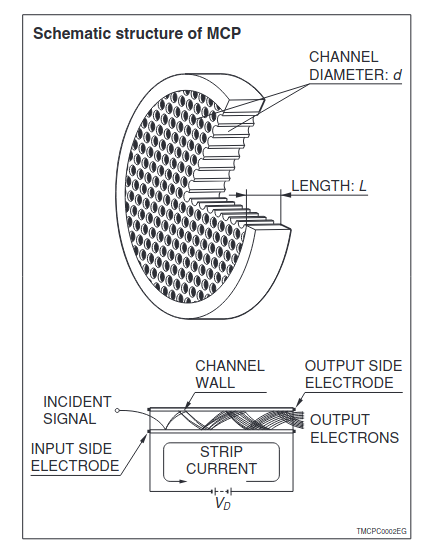
\includegraphics[width=1\linewidth]{Images/TestBeam_setup/MCP diagram HAMAMATSU.png}
\end{minipage}
\hfill
\begin{minipage}[c]{.5\linewidth}
    \caption{
    Schematics of an MCP.\\ 
    Top: structure of the detector with a cross-sectional view of the channels, highlighting the diameter $d$ and the length $L$ of the micro-channels. Standard MCPs are fabricated with a diameter of $10$s \unit{\micro\meter} and a ratio $\alpha$ ($\alpha = L / d$) 40 to 60.\\
    Bottom: when a voltage ($V_D$) is applied, the channel walls behave as continous electron multiplier: when a target object (electron, ion or photon) hits the inner walls, electrons are released in a parabolic trajectory and they start a chain reaction which produces a signal amplified by $10^4-10^7$ times.}
\end{minipage}
\label{fig:MCP_diagrame}
\end{figure}


\subsection{Time resolution of the MCP}
The time resolution of the MCP was first calculated by comparing the time difference of two independent sensors (CNM-W4 and CNM-W5) and the MCP. In this way, it was possible to build a system of three equations of the time differences. 
\begin{equation}\label{eq:time_res_system_eqs}
    \begin{cases}
        t_{1-2} = t_1 - t_2  \\
        t_{1-MCP} = t_1 - t_{MCP} \\
        t_{2-MCP} = t_2 - t_{MCP} \, .
    \end{cases}
\end{equation}

The time distributions (left sides of the equations) were fitted with a gaussian function, each with a width $\sigma_{ij} = \sigma_i \oplus \sigma_j$, where $i$ and $j$ are two of the devices in Equation \ref{eq:time_res_system_eqs} (i.e. MCP, CNM-W4 and CNM-W5). Assuming that the devices were all independent, their time resolutions would also be independent. This gave a system of three equations with three unknowns, which could be solved analytically to find each individual time resolution: $\sigma_1$, $\sigma_2$, $\sigma_{MCP}$.

The results computed this way are shown in Table \ref{tab:MCP_time_resolution}.
\begin{table}[!ht]
    \begin{center}
        \caption{Time resolution values of the MCP. The "Error" is the statistical uncertainty, since the calculation was repeated for all the available runs.}
        \label{tab:MCP_time_resolution}
        \begin{tabular}{ | c | c | c | c | }
            \hline
            Voltage [$\si{V}$] & 2500 & 2600 & 2800 \\ 
            \hline 
            Time resolution [$\si{ps}$] & 36.52 & 16.48 & 3.73 \\  
            Error [$\si{ps}$] & $\pm$0.81 & $\pm$0.57 & $\pm$1.33 \\
            \hline
        \end{tabular}
    \end{center}
\end{table}


\section{Oscilloscopes}
The signal generated by the DUT was recorded by two four-channel oscilloscopes: channel 1 (denoted as Ch1) of both oscilloscopes was connected to the MCP (which was used as time reference, described previously in Section \ref{sec:MCP_description}). So, up to 6 channels were available in each batch to be attached to the DUTs.


\section{The sensors}

There were several samples that were tested, divided into three main categories of design:
\begin{itemize}
    \item USTC, from the University of Science and Technology of China
    \item IHEP, from the Institute of High Energy Physics, China
    \item CNM, from the Centro National de Microelectronica, Barcelona, Spain
\end{itemize}

the first two designs have both been manufactured by the IME (Institute of Microelectronics) of the Chinese Academy of Sciences. The two CNM sensors (labeled CNM-W4 and CNM-W5) were used to measure the time resolution of another device, the MCP (Section \ref{sec:MCP_description}), which was used as a time reference for all of the time measurements of the other LGADs. Table \ref{tab:devices_tested} provides the list of the devices that were characterized, for more detailed descriptions see Table in \nameref{chap:appendix}.



\begin{table}[!ht]
    \centering
    \caption{Summary of the tested devices}
    \label{tab:devices_tested}
    \scriptsize
    % \makebox[1\textwidth][c]{
    \begin{tabularx}{1\textwidth}{|l|l|l|l|l|X|}
    \hline %%% I NEED TO TRY TO USE TABULAR INSTEAD OF SHORTSTACK
        \textbf{Sevice name} & \textbf{Vendor} & \begin{tabular}{@{}l@{}}\textbf{Pads,} \\ \textbf{used channels}\end{tabular} & \begin{tabular}{@{}l@{}}\textbf{Fluence} \\ $[n_{eq}/\si{cm^2}]$ \end{tabular} & \begin{tabular}{@{}l@{}} \textbf{Radiation} \\ \textbf{type} \end{tabular} & \textbf{Notes} \\
        \hline
        CNM-W4  & CNM & single & 0 & - & reference \\ 
        CNM-W5  & CNM & single & 0 & - & reference \\ 
        CNM-W5-1.5E15  & CNM & single & $\num{1.50E+15}$ & neutron &  \\ 
        CNM-W3-2.5E15  & CNM & single & $\num{2.50E+15}$ & neutron &  \\ 
        USTC2.1-W17 & USTC & 2x2, 2 channels  & 0 & - &  \\ 
        USTC2.1-W17-2E14 & USTC & 2x2, 1 channel & 0 & - & missing \\ 
        IMEv3-W12-2x2  & IHEP & 2x2, 2 channels  & 0 & - &  \\ 
        IMEv3-W12-1x3  & IHEP & 1x3, 2 channels  & 0 & - &  \\ 
        IMEv3-W12  & IHEP & 2x2, 3 channels  & $\num{1.50E+15}$ & neutron &  \\ 
        IMEv3-W16  & IHEP & 1x3, 1 channel  & $\num{1.50E+15}$ & neutron &  \\ 
        IMEv2-W7-1E14  & IHEP & single & $\num{1.00E+14}$ & proton &  \\ 
        IMEv2-W7-6.5E14  & IHEP & single & $\num{6.50E+14}$ & proton &  \\ 
        IMEv3-W16-8E14  & IHEP & single & $\num{8.00E+14}$ & proton &  \\
        IMEv3-W16-2.5E15  & IHEP & single & $\num{2.50E+15}$ & neutron &  \\ 
        \hline
    \end{tabularx}
\end{table}